\documentclass{clbeamer2024}

\usepackage{minted}

\usepackage{minted}
\setminted{
	breaklines=true,
	frame=single,
	bgcolor=lightgray,
	fontsize=\small,
	escapeinside=||
}

\usepackage{xcolor}
\definecolor{bg}{rgb}{0.95, 0.95, 0.92} % Couleur gris clair

\title{
	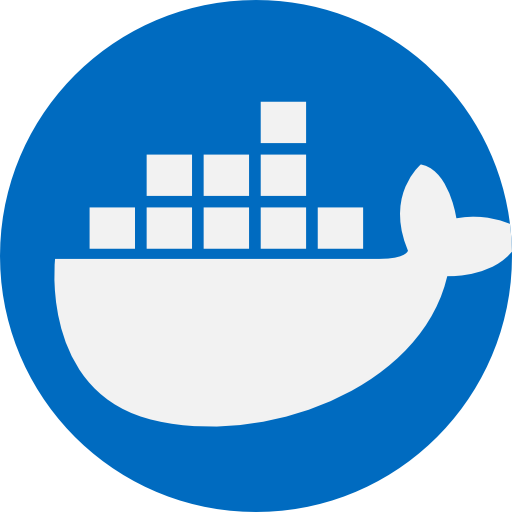
\includegraphics[width=1cm]{logos/docker.png} \hfill
	Introduction aux Conteneurs et à Docker 
}
\subtitle{Comprendre les bases des conteneurs et de Docker}
\author{Slimani Mohamed Amine}
\institute{}
\date{\today}

\begin{document}
	\setcounter{framenumber}{-1}
	\frame{\titlepage}
	
	
	
	% Sommaire
	\begin{frame}{Sommaire}
		\tableofcontents
	\end{frame}
	

\section{Qu'est-ce qu'un conteneur ?}
\begin{frame}{Qu'est-ce qu'un conteneur ?}
	\begin{itemize}
		\item \textbf{Définition} : Un conteneur est une unité logicielle qui encapsule une application et ses dépendances.
		\item \textbf{Avantages} : Isolation, portabilité, légèreté.
		\item \textbf{Comparaison avec les machines virtuelles} : Les conteneurs partagent le noyau du système hôte, ce qui les rend plus légers et plus rapides.
	\end{itemize}
\end{frame}

\section{Qu'est-ce que Docker ?}
\begin{frame}{Qu'est-ce que Docker ?}
	\begin{itemize}
		\item \textbf{Définition} : Docker est une plateforme open-source pour développer, expédier et exécuter des applications dans des conteneurs.
		\item \textbf{Composants} : Docker Engine, Docker Hub, Docker Compose.
		\item \textbf{Avantages} : Simplifie le déploiement, améliore la productivité, facilite la collaboration.
	\end{itemize}
\end{frame}

\section{Concepts de base de Docker}
\begin{frame}{Concepts de base de Docker}
	\begin{itemize}
		\item \textbf{Images} : Modèles en lecture seule pour créer des conteneurs.
		\item \textbf{Conteneurs} : Instances d'exécution d'une image.
		\item \textbf{Volumes} : Persistance des données.
		\item \textbf{Réseaux} : Communication entre conteneurs.
	\end{itemize}
\end{frame}


\section{Cycle de vie d'un conteneur}
\begin{frame}{Cycle de vie d'un conteneur}
	\begin{itemize}
		\item \textbf{Créer une image} : À partir d'un Dockerfile.
		\item \textbf{Lancer un conteneur} : À partir d'une image.
		\item \textbf{Arrêter et redémarrer un conteneur}.
		\item \textbf{Supprimer un conteneur}.
	\end{itemize}
\end{frame}

\section{Dockerfile}
\begin{frame}[fragile]{Dockerfile}
	\begin{exampleblock}{Exemple de Dockerfile}
		\begin{minted}[fontsize=\scriptsize]{dockerfile}
FROM ubuntu:20.04
RUN apt-get update && apt-get install -y python3
COPY . /app
WORKDIR /app
CMD ["python3", "app.py"]
		\end{minted}
	\end{exampleblock}
\end{frame}

\section{Docker Compose}
\begin{frame}[fragile]{Docker Compose}
	\begin{exampleblock}{Exemple de fichier docker-compose.yml}
		\begin{minted}[fontsize=\scriptsize]{yaml}
version: '3'
services:
  web:
    image: nginx
    ports:
      - "80:80"
  db:
    image: postgres
    environment:
      POSTGRES_PASSWORD: example
		\end{minted}
	\end{exampleblock}
\end{frame}

\section{Bonnes pratiques}
\begin{frame}{Bonnes pratiques}
	\begin{itemize}
		\item \textbf{Utiliser des images officielles} : Pour garantir la sécurité et la stabilité.
		\item \textbf{Minimiser la taille des images} : En utilisant des images de base légères et en supprimant les fichiers inutiles.
		\item \textbf{Utiliser des volumes pour les données persistantes} : Pour éviter de perdre des données lors de la suppression d'un conteneur.
	\end{itemize}
\end{frame}

\section{Outils pour travailler avec Docker}
\begin{frame}{Outils pour travailler avec Docker}
	\begin{itemize}
		\item \textbf{Docker CLI} : Interface en ligne de commande pour gérer les conteneurs.
		\item \textbf{Portainer} : Interface graphique pour gérer les conteneurs.
		\item \textbf{Kubernetes} : Orchestration de conteneurs à grande échelle.
	\end{itemize}
\end{frame}

\section{Exemple de commandes Docker}
\begin{frame}[fragile]{Exemple de commandes Docker}
	\begin{exampleblock}{Commandes Docker}
		\begin{minted}[fontsize=\scriptsize]{bash}
# Construire une image
docker build -t mon-image .
			
# Lancer un conteneur
docker run -d -p 80:80 mon-image
			
# Lister les conteneurs en cours d'exécution
docker ps
		\end{minted}
	\end{exampleblock}
\end{frame}

\section{Pourquoi c'est important ?}
\begin{frame}{Pourquoi c'est important ?}
	\begin{itemize}
		\item Les conteneurs et Docker sont essentiels pour le développement moderne et le déploiement d'applications.
		\item Ils améliorent la portabilité, la productivité et la collaboration.
		\item Comprendre leur fonctionnement est crucial pour les développeurs et les administrateurs système.
	\end{itemize}
\end{frame}

\begin{frame}{Résumé}
	\textbf{Les conteneurs et Docker} sont des technologies clés pour le développement et le déploiement d'applications modernes. Ils offrent isolation, portabilité et légèreté. 🐳
\end{frame}


	
	
\end{document}
